\section{Hybrid 8-bit Floating-Point and 4-bit Logarithmic Computation}
\tableofcontents[currentsection]

\begin{frame}{Spike-by-Spike Neural Network}
	\begin{columns}[c]  % Top alignment for the columns
		
		% Left Column for top left image
		\begin{column}{0.5\textwidth}
			\uncover<1->{  % Uncover the top left image first
				\begin{figure}
					\centering
					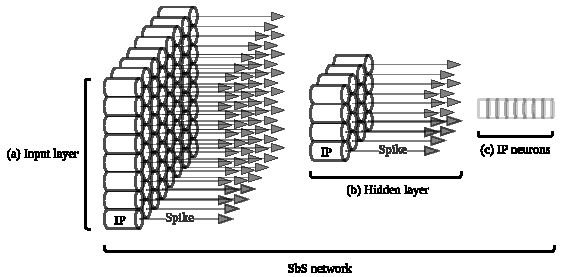
\includegraphics[width=\textwidth]{../chapters/sbs_accelerator/figures/SbS_layer.pdf}
					\caption{SbS inference}
				\end{figure}
			}
		\end{column}
		
		% Right Column for top right image
		\begin{column}{0.5\textwidth}
			\uncover<2->{  % Uncover the top right image second
				\begin{figure}
					\centering
					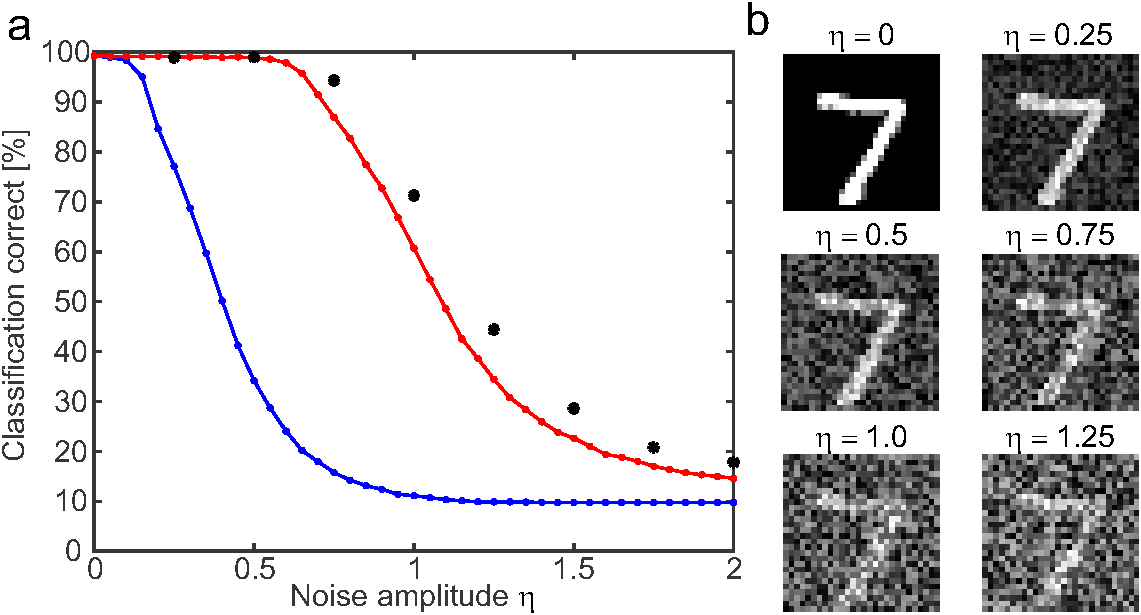
\includegraphics[width=0.9\textwidth]{../chapters/sbs_accelerator/figures/sbs_robustnes.pdf}
					\caption{Robustness of SbS NN versus CNN}
				\end{figure}
			}
		\end{column}
		
	\end{columns}
	\vspace{10mm}
	% Bottom full-width equation
	\uncover<3->{  % Uncover the equation last across the full width of the slide
		\[
		h_\mu^{new}(i) = \frac{1}{1+\epsilon} \left(h_\mu(i) + \epsilon \frac{h_\mu(i) W(s_t|i) }{\sum_j h_\mu(j) W(s_t|j)} \right) 
		\]
	}
\end{frame}

\begin{frame}{HW/SW Co-Design and Deployment Framework}

			\begin{figure}
				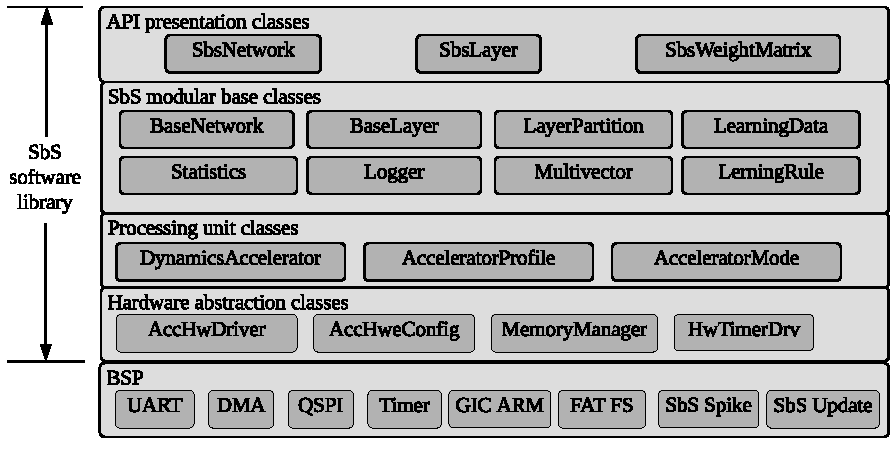
\includegraphics[width=0.75\textwidth]{slides/figures/sbs_software_component.pdf}
				\caption{System-level overview of the embedded software architecture}
			\end{figure}

\end{frame}
